\documentclass{article}
\usepackage{graphicx} % Required for inserting images
\usepackage{algorithm}
\usepackage{amsmath}
\usepackage{amssymb}
\usepackage{tikz}
\title{FFT using topelitz Matrix embedded in a Larger Circulent Matrix via Convolution Theoram}
\author{
Kartik Ohlan \\
Instructor: Professor Johnson
}
\date{March 2026}

\begin{document}

\maketitle

\section{Fundamentals:}

For FFT to be defined, we first talk about basic identities we will use:

a) $$1 + \omega + \omega^2 =0$$
    where $$\omega = e^{i\frac{2\pi}{3}}$$ defines \textbf{n-th root unity}
    and we know in order to calculate $$e^{i\frac{2\pi}{3}}$$ we use the following equation:
    $$e^{i\frac{2\pi}{3}}$$ = $$ cos \frac{2\pi}{3} + sin\theta \frac{2\pi}{3}$$
b)  \[
\text{Conjugate:} \quad a + ib \longrightarrow a - ib
\]
    So from our roots of unity we would have:


\section{Proof of Convolution}

Now we work towards proving \[f_n \, (x \circledast y) = f_n(x) \cdot f_n(y) \equiv f_n \, \text{diagonlize} \,  C_{x} \]

In this proof we consider the shift matrix $S_3$ which represent the cyclic matrix

\[D_3 F_3 \equiv  S_3 \cdot F_x\]

Multiplying both sides on the right by $F_3^{-1}$ gives,

\begin{center}
\begin{equation}
D_3 = S_3 \cdot F_3 \cdot F_3^{-1}
\label{eq:c3}
\end{equation}
\end{center}


we have \[F_3 = \begin{bmatrix} 1&1&1 \\ 1 & \omega & \omega^2  \\1 & \omega^2 & \omega \end{bmatrix}\] 

and \[F_3^{-1} = \begin{bmatrix} 1&1&1 \\ 1 & \omega^2 & \omega \\ 1 & \omega &     \omega^2 \end{bmatrix}\]

\textbf{From the unit circle we observe that the three roots are separated by an angle of 120°.}
\begin{center}
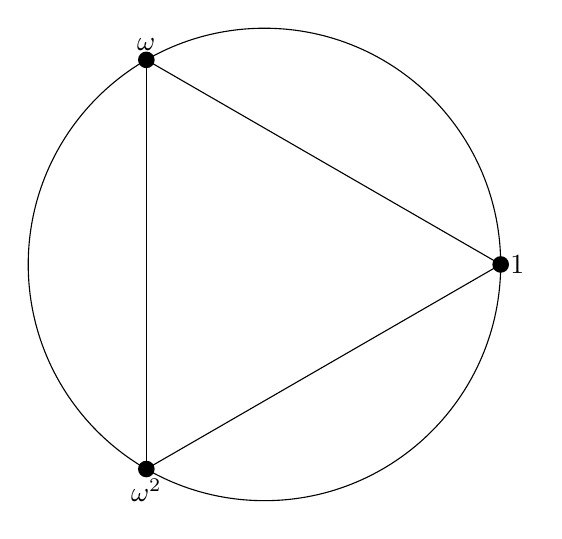
\begin{tikzpicture}

\draw (0,0) circle (3);

\fill (3,0) circle (3pt) node[right] {$1$};
\fill (-1.5,2.598) circle (3pt) node[above] {$\omega$};
\fill (-1.5,-2.598) circle (3pt) node[below] {$\omega^2$};
\draw[->] (3,0) -- (-1.5,2.598);
\draw[->] (-1.5,2.598) -- (-1.5,-2.598);
\draw[->] (-1.5,-2.598) -- (3,0);
\end{tikzpicture}
\end{center}

Moving counter-clockwise on this unit circle will give following structure:

$1$ \cdot $\omega$ = $\omega$

$\omega \cdot \omega = \omega^2$

$\omega \cdot \omega^2 = \omega^3 == 1$


\subsection{Circular Convolution}
lets say we have an input vector $\textbf{x = [x0 \, x1 \,x2]}$

The Circular matrix corresponding to a right shift is

\[C_3  = \begin{bmatrix}
    x_0 &  x_1 & x_2 \\ x_2 & x_0 & x_1 \\ x_1 & x_2 & x_0
\end{bmatrix}\]

Now we take a matrix $D_3$ which is defined as: $D_3 \xrightarrow{} (1,\omega,\omega^2)$

Now, if we look closely $C_3$ matrix is nothing but Linear Combination of power of shift matrix:

\begin{equation}
C_x = x_0I_3 + x_1S_3 + x_2S_3^2
\label{eq:C_x}
\end{equation}
if we look closely $I_3 = S_3^0$

where 
\[D_3^0 = \begin{bmatrix}
    1 & 0 & 0 \\ 0 & 1 & 0 \\  0 & 0 & 1
\end{bmatrix}\]

From equation 1 and 2 we can use subsitiution

\[FC_xF^-1 = F_3(x_0 I_3+x_1S_3^1 + x_2S_3^2)F_3^{-1}\]

multiplying:

\[F_3C_3F_3^-1 = x_0(F_3I_3F_3^{-1})+x_1(F_3S_3^1F_3^{-1}) + x_2(F_3S_3^2F_3^{-1})\]

by substituting eq 1 it becomes,

\[F_3C_3F_3^-1 =  x_0I_3 + x_1D_3^{1} + x_2D_3^{2} \]

which proves,
\[F_n C_xF_n^{-1} \equiv diag(F_nx) \]


\subsection{Concepts on Convolution}
To be mindfull, we can have cyclic in both down and upshift direction.

$\text{Downshift} \longrightarrow \text{left-shift on } I_n$
Proof:
[\lets say we have input vector (g) 


\subsection{Cooley - Tookey's Method (for general form)}
This section will talk about the one of the ways FFT in order calculate DFT's

We know for for general dft we have

\[
y_k = \sum_{n=0}^{N-1} x_n \, \omega_N^{k n}
\]

Now we take $N = R \cdot S$.

where $R$ and $S$ are the factors of $N$.

Let $\omega_N$ denote a primitive $N$th root of unity.
For the $4 \times 4$ example below, we use $\omega_4 = i$, where $i^2 = -1$.

\[\]

Now  for any F_n matrix we can have 
\[D_n = \begin{bmatrix}
    \omega^{i.j}  & \omega^{i.j+1}    & \omega^{i.j+2}   & \omega^{i.j+3}  \\ \omega^{i+1.j}   & \omega^{i+1.j+1}  & \omega^{i+1.j+2} & \omega^{i+1.j+3}   \\  \omega^{i+2.j}  & \omega^{i+2.j+1}  & \omega^{i+2.j+2} & \omega^{i+2.j+3}  \\ \omega^{i+3.j}  & \omega^{i+3.j+1}  & \omega^{i+3.j+2}  & \omega^{i+3.j+3} 
\end{bmatrix}\]

which if we take a 4*4 example then we have 

\[C_4  = \begin{bmatrix}
    1 &  1 & 1 & 1 \\ 1 & i & -1 & -i \\ 1 & -1 & 1 & -1 \\ 1 & -i & -1 & i 
\end{bmatrix}\]

\begin{align}
y_0 &= x_0 + x_1 + x_2 + x_3 \\
y_1 &= x_0 + i \cdot x_1 - x_2 - i \cdot x_3 \\
y_2 &= x_0 - x_1 + x_2 - x_3 \\
y_3 &= x_0 - i \cdot x_1 - x_2 + i \cdot x_3
\end{align}

For a general DFT we have:
\begin{itemize}
    \item Multiplications: $N^2$
    \item Additions: $N(N-1)$
\end{itemize}

Please note that when we say additions, we also include subtractions, since
\[
a - b = a + (-b).
\]

So in this case we have 16 FLOPs.
\textbf{Now we can already see the runtime O(n^{2})}

\end{document}
